%   LaTeX template for Beijing Jiaotong University thesis
%
%   -*- coding: utf-8 -*-
%
%   File Name : bjtuthesis.tex
%
%   Usage : Main file entry
%
%   Creation Date : 2025-05-13
%
%   Last Modified : 2025-06-22
%
%   Author : PangSMPang (pangsmpang325@gmail.com)

% If you encounter issues while using this template, please try the following:
%   1. Refer to the online documentation provided earlier to check for potential solutions.
%   2. Browse the GitHub Issue list to see if your problem has already been addressed.
%   3. If needed, create a new GitHub Issue to report or discuss the problem with me.

\documentclass[
    TwoSide = false, % set to false if you don't need empty pages
    BlindReview = false, % set to true if you need to hide personal information
    NumberByChapter = false, %set to true if you need to number by chapter
]{bjtuthesis}
\setcounter{gbrefcompress}{4} %在同一处引用多篇序号连续的文献时,标注标签默认是从两篇文献开始压缩的,gbrefcompress 的值为 4,则4篇以上才压缩,引用编号将以逗号分隔,例如 [1,2,3],而不是 [1–3],如何设置看个人喜好
\captionsetup[table]{labelsep=space}%设置正文表的分隔符可选参数space:空格 colon:冒号 period:点 quad:长空格
\captionsetup[figure]{labelsep=space}%设置正文图的分隔符可选参数space:空格 colon:冒号 period:点 quad:长空格
%========================================================================%
% 自定义内容
%========================================================================%
\author{张三}
\studentNumber{100044}
\advisor{李四}
\department{计算机科学与技术学院}
\major{计算机科学与技术}
\title{ 毕业论文(设计)题目}
\englishtitle{Title of Project (Thesis)}


\begin{document}
\pagestyle{empty} 
\makecover % 封面
%========================================================================%
% 两个声明
%========================================================================%
\makeatletter
\ifbjtuthesis@BlindReview
  % 盲审模式
\else
  % 非盲审模式:正常载入这两个文件
  \cleardoublepage{}

\thispagestyle{fancynofoot}
\markboth{版权使用授权书}{}
\vspace*{-0.53cm}
\begin{center}
{\zihao{-2}\heiti 学士论文版权使用授权书\bigskip}
\end{center}

本学士论文作者完全了解北京交通大学有关保留、使用学士论文的规定。特授权北京交通大学可以将学士论文的全部或部分内容编入有关数据库进行检索,提供阅览服务,并采用影印、缩印或扫描等复制手段保存、汇编以供查阅和借阅。\\
\vspace{-0.4cm}
\begin{center}
(保密的学位论文在解密后适用本授权说明)
\end{center}
\vspace{3cm}

\begin{minipage}[t]{0.5\textwidth}
学位论文作者签名:\vspace{4ex}

签字日期:\hspace{2em}年\hspace{2em}月\hspace{2em}日
\end{minipage} 
\hfill
\begin{minipage}[t]{0.5\textwidth}
指导教师签名:\vspace{4ex}

签字日期:\hspace{2em}年\hspace{2em}月\hspace{2em}日
\end{minipage} 	
\cleardoublepage{}
 % 版权声明
  \cleardoublepage{}

\thispagestyle{fancynofoot} 
\markboth{论文诚信声明}{}
\vspace*{-0.53cm}
\begin{center}
{\zihao{-2}\heiti 学士论文诚信声明\bigskip}
\end{center}

本人声明所呈交的毕业论文(设计),题目\uline{\title}是本人在指导教师的指导下,独立进行研究工作所取得的成果。尽我所知,除了文中特别加以标注和致谢中所罗列的内容以外,论文中不包含其他人已经发表或撰写过的研究成果,也不包含为获得北京交通大学或其他教育机构的学位或证书而使用过的材料。

申请学位论文与资料若有不实之处,本人承担一切相关责任。\\

本人签名:\underline{\makebox[10em]{}} \qquad 日期:\underline{\makebox[10em]{}}                
\newpage   % 诚信声明
\fi
\makeatother
%========================================================================%
% 摘要部分
%========================================================================%
\setcounter{page}{1}
\pagenumbering{roman}
\pagestyle{bjtufancy}

\cleardoublepage{}

\begin{chineseabstract}	

\noindent{\textbf{摘要:}}
中文摘要应将论文的内容要点简短明了地表达出来,约400字左右,字体为宋体小四号。内容应包括工作目的、研究方法、成果和结论。要突出本论文的创新点,语言力求精炼。为了便于文献检索,应在本页下方另起一行注明论文的关键词(3-5个),如有可能,尽量采用《汉语主题词表》等词表提供的规范词。图X幅,表X个,参考文献X篇。

{
    \vspace{2cm}
    \noindent
    \textbf{关键词:} 关键词 1 ; 关键词 2; 关键词 3 \par %请替换关键词(3-5个),以分号分隔。
}
	
	
	
	
	
	
	
	
	
\end{chineseabstract}
 % 中文摘要
\cleardoublepage{}

\begin{englishabstract}

\noindent{\textbf{ABSTRACT:}} 
与中文摘要内容要相对应
	

{
    \vspace{2cm}
    \noindent
    \textbf{KEYWORDS:}  keyword 1 ; keyword 2 ;keyword 3\par  %请替换关键词(3-5个),与中文关键词保持一致,以分号分隔。]
}





\end{englishabstract} % 中文摘要

% 目录
\tableofcontents
\cleardoublepage
%========================================================================%
% 主体部份
%========================================================================%

\newpage
\pagestyle{bjtufancymain}
\setcounter{page}{1}
\pagenumbering{arabic}

\cleardoublepage{}

\chapter{绪论}
引言(或绪论)简要说明研究工作的目的、范围、相关领域的前人工作和知识空白、理论基础和分析、研究设想、研究方法和实验设计、预期结果和意义等。应言简意赅,不要与摘要雷同,不要成为摘要的注释。一般教科书中有的知识,在引言中不必赘述。

\section{编译方式说明}

\subsection*{在 Overleaf 上编译}

请注意以下事项:

\begin{itemize}
  \item 请上传整个 \verb|.zip| 压缩包。
  \item 不要删除 \verb|.latexmkrc| 文件,Overleaf 会自动识别并使用 XeLaTeX 编译(你也可以手动设置为 XeLaTeX)。
  \item 在 \verb|chapter| 文件夹下编辑你的各章节内容。
\end{itemize}

\subsection*{在本地编译}

请按照以下步骤操作:

\begin{itemize}
  \item 打开主 \verb|.tex| 文件,例如:\verb|bjtuthesis.tex|。
  \item 进入:选项 $\rightarrow$ 设置 TexStudio $\rightarrow$ 构建,设置如下:
    \begin{itemize}
      \item 默认编译器选择:\verb|XeLaTeX|
      \item 默认文献工具选择:\verb|Biber|
    \end{itemize}
  \item 点击工具栏绿色箭头“构建 \& 查看”(或按 \verb|F5|)。
  \item 如果文献未显示,点击顶部菜单“工具(T)” $\rightarrow$ “参考文献(B)”运行 Biber(或按 \verb|F8|)。
  \item 然后运行 XeLaTeX 两次,即点击两次“构建 \& 查看”(\verb|F5|)。
\end{itemize}

\vspace{1em}
\noindent 快捷方式:设置完成后,按顺序使用快捷键 \verb|F5 - F8 - F5 - F5| 即可完整编译。

\subsection*{在服务器(Linux)编译}

建议使用 \verb|Makefile|,集成了编译、清理中间文件、打开 PDF 三个步骤。

注意:使用 \verb|Makefile| 时请勿修改主 \verb|.tex| 文件名。

可用命令如下:

\begin{itemize}
  \item \verb|make|:等同于 \verb|make all|,执行清理后编译 PDF。
  \item \verb|make bjtuthesis|:仅编译 PDF。
  \item \verb|make clean|:仅清理中间文件。
  \item \verb|make view|:仅打开生成的 PDF。
\end{itemize}


\section{统计字数脚本}

模板提供了统计字数脚本,可在服务器或本地运行:

\subsection*{使用 Bash 运行 \texttt{word\_count.sh}}

\begin{enumerate}
  \item 打开终端(Windows 推荐使用 Git Bash 或 WSL + VS Code),切换到项目目录:
  
  \begin{verbatim}
cd path\to\your\project
  \end{verbatim}

  \item 执行脚本,传入主 \verb|.tex| 文件名:
  
  \begin{verbatim}
./scripts/word_count.sh bjtuthesis.tex
  \end{verbatim}

  \item 输出说明:
  \begin{itemize}
    \item 控制台显示简要统计信息;
    \item 完整统计信息输出至:\verb|outputs/bjtuthesis.wordcnt|。
  \end{itemize}
\end{enumerate}

\subsection*{使用 PowerShell 运行 \texttt{word\_count.ps1}}

\begin{enumerate}
  \item 打开终端,切换到项目目录:

  \begin{verbatim}
cd path\to\your\project
  \end{verbatim}

  \item 执行脚本,传入主 \verb|.tex| 文件名:

  \begin{verbatim}
./scripts/word_count.ps1 bjtuthesis.tex
  \end{verbatim}

  \item 输出说明:
  \begin{itemize}
    \item 控制台显示简要统计信息;
    \item 完整统计信息输出至:\verb|outputs/bjtuthesis.wordcnt|。
  \end{itemize}
\end{enumerate}


\cleardoublepage{}

\chapter{相关技术}



\section{插入说明}

我们可以用 includegraphics 来插入现有的不同格式的图片,如图\ref{fig:ai-agent}。论文中尽量使用矢量图,如.pdf格式的图片

\begin{figure}[ht]
    \centering
    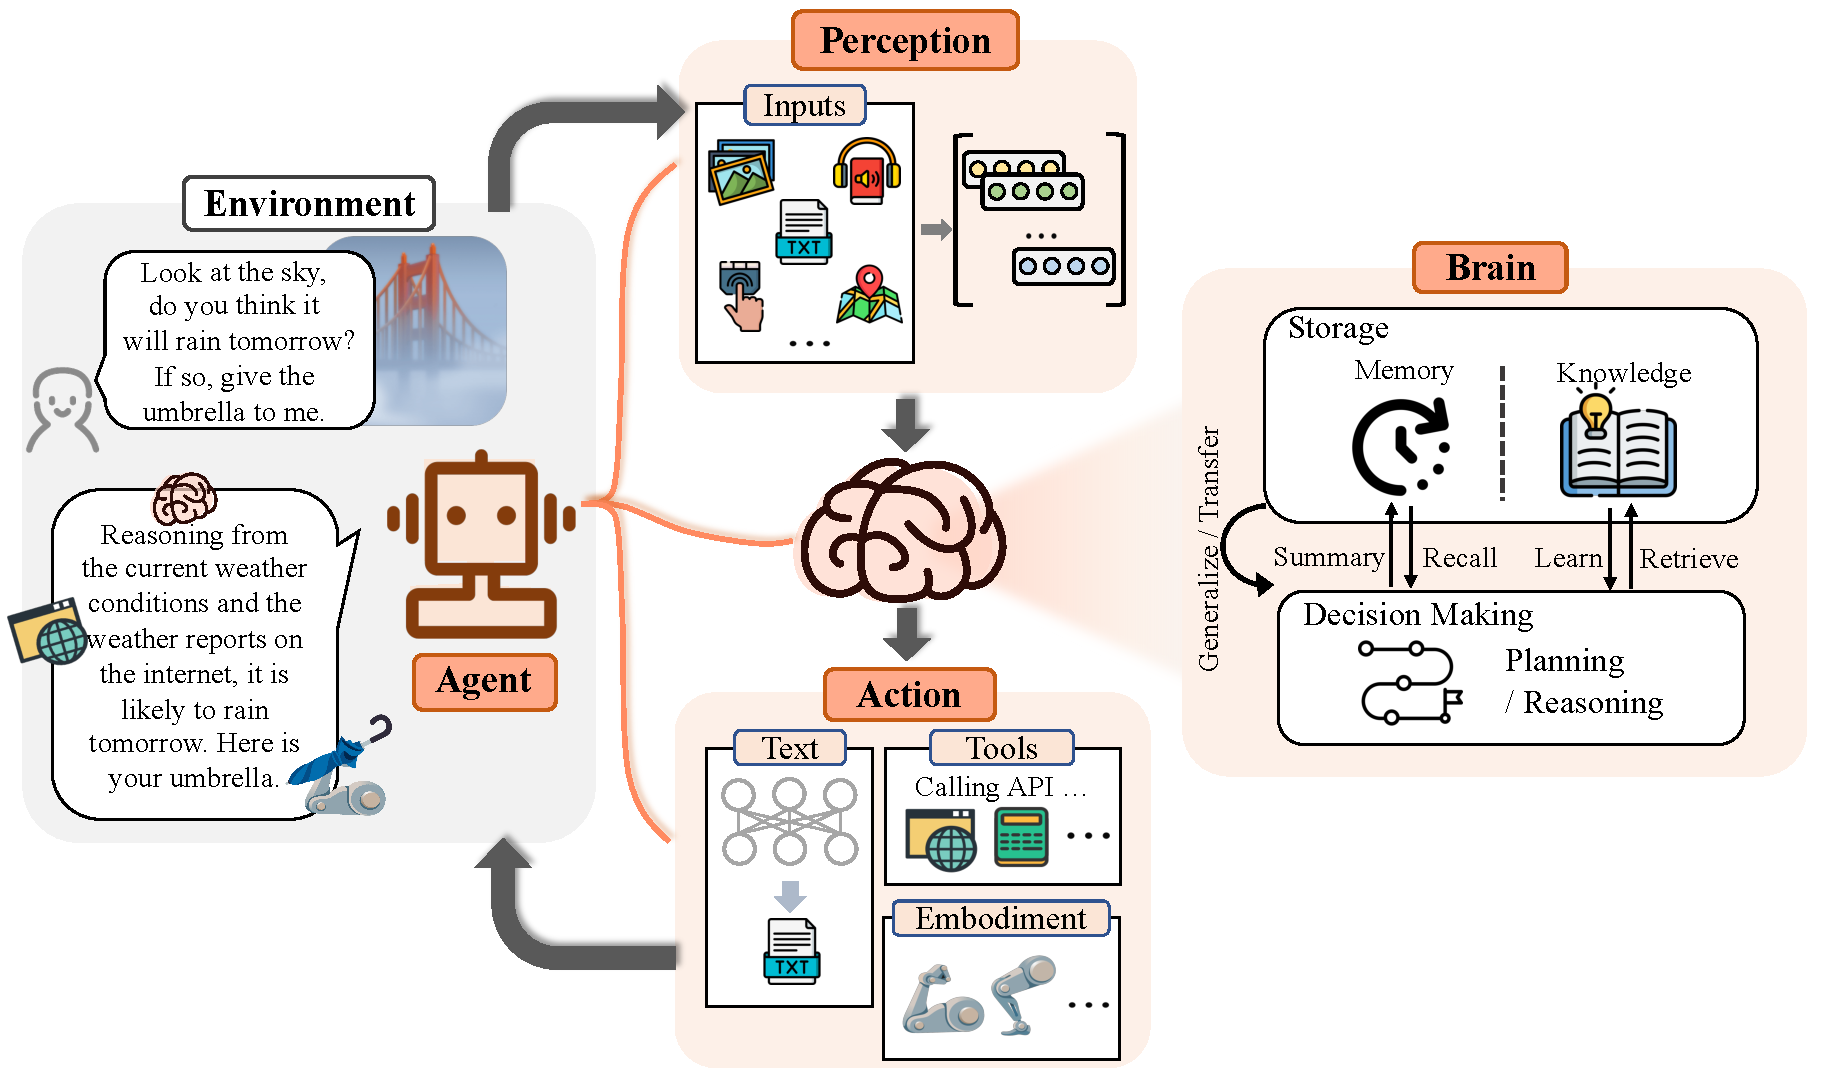
\includegraphics[width=.4\linewidth]{AI agent的组成.pdf}
    \caption{\label{fig:ai-agent}AI agent的组成.pdf}
\end{figure}

\par 如\ref{tab:compare}所示,这是一张自动调节列宽的表格。推荐两个常用的在线表格生成工具:Advanced Table Editor(\url{https://www.latex-tables.com/})和 Tables Generator(\url{https://www.tablesgenerator.com/})。


\begin{table}[ht]
	\footnotesize           
	\centering
	\caption{代码智能体相比 Text/JSON 在 LLM 动作上的优势}
	\label{tab:compare}
	\setlength\extrarowheight{2pt}  % 适度增大行距
	\begin{tabularx}{\textwidth}{lXX}
		\toprule
		& \textbf{代码智能体用于 LLM 动作} & \textbf{JSON 或 Text 用于 LLM 动作} \\
		\midrule
		预训练数据兼容性 & 有大量代码可用于预训练 & 需要针对特定格式进行数据整理 \\
		复杂操作支持 & 通过控制流和数据流原生支持 & 即便可行,也需要精心设计(例如定义新工具以模拟 if 语句) \\
		工具可用性 & 可以直接使用现有的软件包 & 需手动适配工具 \\
		自动反馈能力 & 反馈机制(如 traceback)作为基础机制已经在大多数编程语言中实现 & 需额外设计反馈流程 \\
		\bottomrule
	\end{tabularx}
\end{table}

\par 如\ref{equ:sample},这是一个公式

\begin{equation}
\label{equ:sample}
\mathrm{Logits}(t_n) = \mathrm{GenModel}\bigl(t_n \mid \{\mathrm{input}, t_1, \ldots, t_{n-1}\}\bigr)
\end{equation}

\par 如算法\ref{alg:sample},这是一个算法

\begin{algorithm}[ht]
	\caption{CodeAgent-based Workflow}
	\label{alg:sample}
	\begin{algorithmic}
		\State \textbf{memory} $\gets$ [user\_defined\_task]
		\While{llm\_should\_continue(memory)}
		\State $action \gets llm\_get\_next\_action(memory)$
		\State $observations \gets execute\_action(action)$
		\State $memory \gets memory + [action,\ observations]$
		\EndWhile
	\end{algorithmic}
\end{algorithm}

\par 这是一个无序列表

\begin{itemize}
    \item aaa
    \item bbb
    \item ccc
\end{itemize}

\par 这是一个有序列表(默认编号格式)

\begin{enumerate}
    \item aaa
    \item bbb
    \item ccc
\end{enumerate}

\par 下面是两个有序列表(自定义编号格式),你可以按照你的偏好设置

\begin{enumerate}[label=\arabic*)]	
    \item aaa
    \item bbb
    \item ccc
\end{enumerate}

\noindent\hrulefill

\begin{enumerate}[label=(\alph*)]
    \item athesiaa
    \item bbb
    \item ccc
\end{enumerate}

\subsection{文献引用}

文献引用可以使用两种方式,下面两种方式任选一个即可,但是需要全文统一

引用文献方式一:文献\cite{Chase_LangChain_2022}、文献\cite{wang2024executable}

引用文献方式二:文献\parencite{Elovic_gpt-researcher_2023}、文献\parencite{smolagents}

\subsection{关于代码}

\par 目前学院没有明确给出代码格式,你可以自己定义,也可以参照我的设置来使用
\begin{verbatim}
%复制以下代码到导言区
\definecolor{dkgreen}{rgb}{0,0.6,0}
\definecolor{gray}{rgb}{0.5,0.5,0.5}
\definecolor{mauve}{rgb}{0.58,0,0.82}

\lstset{ 
    language=python,                
    basicstyle=\footnotesize,       
    numbers=left,                   
    numberstyle=\tiny\color{gray}, 
    stepnumber=1,                   
    numbersep=5pt,                  
    backgroundcolor=\color{white}, 
    showspaces=false,              
    showstringspaces=false,         
    showtabs=false,                 
    frame=single,                   
    rulecolor=\color{black},        
    tabsize=2,                      
    captionpos=b,                   
    breaklines=true,                
    breakatwhitespace=false,        
    title=\lstname,                   
    keywordstyle=\color{blue},          
    commentstyle=\color{dkgreen},       
    stringstyle=\color{mauve},         
    escapeinside={\%*}{*)},            
    morekeywords={*,...}               
}
\end{verbatim}

\definecolor{dkgreen}{rgb}{0,0.6,0}
\definecolor{gray}{rgb}{0.5,0.5,0.5}
\definecolor{mauve}{rgb}{0.58,0,0.82}

\lstset{ 
    language=python,                
    basicstyle=\footnotesize,       
    numbers=left,                   
    numberstyle=\tiny\color{gray}, 
    stepnumber=1,                   
    numbersep=5pt,                  
    backgroundcolor=\color{white}, 
    showspaces=false,              
    showstringspaces=false,         
    showtabs=false,                 
    frame=single,                   
    rulecolor=\color{black},        
    tabsize=2,                      
    captionpos=b,                   
    breaklines=true,                
    breakatwhitespace=false,        
    title=\lstname,                   
    keywordstyle=\color{blue},          
    commentstyle=\color{dkgreen},       
    stringstyle=\color{mauve},         
    escapeinside={\%*}{*)},            
    morekeywords={*,...}               
}
上述设置最后生成的代码样式如下:

Java代码示例:
\begin{lstlisting}[language=java]
private void parseJSONWithJSONObject(String jsonData,SQLiteDatabase db){
    try {
        JSONObject jsonObject = new JSONObject(jsonData);
        JSONArray results;
        if(jsonObject.has("result")) results = jsonObject.getJSONArray("result");  // 获取名为 "result" 的 JSON 数组
        else return;;
        for (int i = 0; i < results.length(); i++) {
            JSONObject item = results.getJSONObject(i);
            String name = item.optString("name");  // 使用 optString 防止 null 引起程序崩溃
            String img = item.optString("img");
            String heat = item.optString("heat");
            String pinyin = getFullPinyin(name);
            if(name.length()>10||name=="null") continue;
            int calor=extractCalories(heat);
            try {
                String sql = "INSERT INTO food (foodname, img, calories, unit, pinyin) VALUES ('" + name + "', '" + img + "', " + calor + ", '100', '" + pinyin + "')";
                db.execSQL(sql);
                Log.d("We", "Insert successful: foodname " + name + ", img " + img + ", heat " + calor +  ", pinyin " + pinyin);
            } catch (SQLException e) {
                Log.e("We", "Insert failed: " + e.getMessage());// 处理插入失败的情况
            }
        }
    }
    catch(Exception e){
        Log.d("Fooddatabase failed","failed",e);
        e.printStackTrace();
    }
}
\end{lstlisting}	

Python代码示例:
\begin{lstlisting}[language=python]
 def generate_with_cue_words(self, background: str):
        problem, message_input = self.api_helper.generate_problem_with_cue_words(
            background, self.paper_list, self.cue_words
        )
        idea = self.api_helper.generate_idea_with_cue_words(
            problem, self.paper_list, self.cue_words
        )
        idea_filtered = self.api_helper.filter_idea(idea, background)
        return message_input, problem, idea, idea_filtered

\end{lstlisting}	
\cleardoublepage{}

\chapter{基本方法}
1级标题内容

\section{2级标题}
2级标题内容

\subsection{3级标题}
3级标题内容
\cleardoublepage{}

\chapter{实验}
1级标题内容

\section{2级标题}
2级标题内容

\subsection{3级标题}
3级标题内容
\cleardoublepage{}

\chapter{结论}

论文的结论是最终的、总体的结论,不是正文中各段的小结的简单重复。结论应该准确、完整、明确、精练。如果不可能导出应有的结论,也可以没有结论而进行必要的讨论。可以在结论或讨论中提出建议、研究设想、仪器设备改进意见以及尚待解决的问题等。

\section{总结}


\section{展望}



%========================================================================%
% 参考文献
%========================================================================%
\newpage
\pagestyle{bjtufancy}
\printbibliography[heading=bjtuheading]
\addcontentsline{toc}{part}{参考文献}
%========================================================================%
% 致谢
%========================================================================%
\makeatletter
\ifbjtuthesis@BlindReview
    % 盲审模式
\else
    \cleardoublepage{}

\begin{acknowledgement}
放置在参考文献页后,对象包括:1)国家科学基金,资助研究工作的奖学金基金,合同单位,资助或支持的企业、组织或个人。2)协助完成研究工作和提供便利条件的组织或个人。3)在研究工作中提出建议和提供帮助的人。4)给予转载和引用权的资料、图片、文献、研究思想和设想的所有者。5)其他应感谢的组织和个人。



\end{acknowledgement}

\fi
%========================================================================%
% 附录
%========================================================================%     
\cleardoublepage{}
\appendix
\pagestyle{bjtufancyappendix}
\appendixfront

\chapternopagebreak{程序代码} %附录的每一章都需要用这个命令,否则会自动分页
附录是作为论文主体的补充项目,并不是必须的。

\chapternopagebreak{工程图纸} %附录的每一章都需要用这个命令,否则会自动分页



\end{document}
